
\de{ĐỀ THI GIỮA HỌC KỲ I NĂM HỌC 2023-2024}{THPT Tân Bình}
\begin{center}
	\textbf{PHẦN 1 - TRẮC NGHIỆM}
\end{center}
\Opensolutionfile{ans}[ans/ans]

%Câu 1
\begin{ex}%[0D3B1-3]%[Dự án đề kiểm tra Toán 10 GHKI NH23-24-Đoàn Minh Tâm]%[THPT Tân Bình - TP. Hồ Chí Minh]
	Tập giá trị $T$ của hàm số $f(x)=\heva{&-1&, \text{khi }x<0\\&1&, \text{khi }x>0}$ là
	\choice
	{\True $T=\{-1 ; 1\}$}{$T=\mathbb{R} \backslash\{0\}$}{$T=(-1 ; 1)$}{$T=[-1 ; 1]$}
	\loigiai{
		Ta có tập giá trị là $T=\{-1;1\}$.
	}
\end{ex}

%Câu 2
\begin{ex}%[0D1Y2-3]%[Dự án đề kiểm tra Toán 10 GHKI NH23-24-Đoàn Minh Tâm]%[THPT Tân Bình - TP. Hồ Chí Minh]
	Cho tập hợp $A=\{x \in \mathbb{R} \mid -1 \leq x<2\}$. Khẳng định nào sau đây đúng?
	\choice
	{\True $A=[-1 ; 2)$}{$A=[-1 ; 2]$}{$A=\{-1 ; 0 ; 1\}$}{$A=\{-1 ; 0 ; 1 ; 2\}$}
	\loigiai{
		Ta có  $A=[-1 ; 2)$.
	}
\end{ex}

%Câu 3
\begin{ex}%[0D1Y2-2]%[Dự án đề kiểm tra Toán 10 GHKI NH23-24-Đoàn Minh Tâm]%[THPT Tân Bình - TP. Hồ Chí Minh]
	Cho tập hợp $A=\{a ; b ; c\}$. Khẳng định nào sau đây \textbf{SAI}?
	\choice
	{$A \subset A$}{\True $a \subset A$}{$\{b ; c\} \subset A$}{$\varnothing \subset A$}
	\loigiai{
		Phần tử không phải là tập con của $A$ được nên $a \subset A$ sai.
	}
\end{ex}

%Câu 4
\begin{ex}%[0D2Y1-2]%[Dự án đề kiểm tra Toán 10 GHKI NH23-24-Đoàn Minh Tâm]%[THPT Tân Bình - TP. Hồ Chí Minh]
	Điểm nào sau đây thuộc miền nghiệm của bất phương trình $3 x+2 y-4>0$?
	\choice
	{\True $P(-1 ; 5)$}{$N(1 ;-1)$}{$M(1 ; 0)$}{$Q(0 ; 2)$}
	\loigiai{
		Ta có $3\cdot (-1)+2\cdot 5-4=3>0$.
	}
\end{ex}

%Câu 5
\begin{ex}%[0H4B1-3]%[Dự án đề kiểm tra Toán 10 GHKI NH23-24-Đoàn Minh Tâm]%[THPT Tân Bình - TP. Hồ Chí Minh]
	Cho tam giác $ABC$. Mệnh đề nào sau đây đúng?
	\choice
	{$\tan (A+B)=\tan C$}{$\cot (A+C)=\cot B$}{\True $\sin (A+B)=\sin C$}{$\cos (A+B)=\cos C$}
	\loigiai{
		Ta có $\sin(A+B)=\sin(180^\circ-C)=\sin C$.
	}
\end{ex}

%Câu 6
\begin{ex}%[0H4Y2-2]%[Dự án đề kiểm tra Toán 10 GHKI NH23-24-Đoàn Minh Tâm]%[THPT Tân Bình - TP. Hồ Chí Minh]
	Cho tam giác $A B C$ có $B C=a$; $C A=b$; $A B=c$. Gọi $S$, $R$, $p$ lần lượt là diện tích, bán kính đường tròn ngoại tiếp và nửa chu vi của tam giác $A B C$. Khẳng định nào sau đây là đúng?
	\choice
	{\True $a^2=b^2+c^2-2 b c \cos A$}{$S=\sqrt{p(p+a)(p+b)(p+c)}$}{$b=\dfrac{2 R}{\sin B}$}{$S=b c \sin A$}
	\loigiai{
		$a^2=b^2+c^2-2 b c \cos A$ đúng vì đây là định lý cosin.
	}
\end{ex}

%Câu 7
\begin{ex}%[0D1Y1-2]%[Dự án đề kiểm tra Toán 10 GHKI NH23-24-Đoàn Minh Tâm]%[THPT Tân Bình - TP. Hồ Chí Minh]
	Trong các câu sau, câu nào là mệnh đề đúng?
	\choice
	{$2 x+1=3$}{$8$ là số nguyên tố}{\True $105$ chia hết cho $3$}{$104$ không chia hết cho $4$}
	\loigiai{
		$105$ chia hết cho $3$.
	}
\end{ex}

%Câu 8
\begin{ex}%[0D3Y1-2]%[Dự án đề kiểm tra Toán 10 GHKI NH23-24-Đoàn Minh Tâm]%[THPT Tân Bình - TP. Hồ Chí Minh]
	Xét hàm số $y=f(x)$ xác định bởi bảng sau
	\begin{center}
		\renewcommand\arraystretch{1.8} %độ rộng của hàng
		\begin{tabular}{|c|c|c|c|c|c|}
			\hline
			$x$&$1$&$2$&$3$&$4$&$5$ \\
			\hline
			$f(x)$&$9$&$6$&$7$&$8$&$10$\\
			\hline
		\end{tabular}
	\end{center}
	Tập xác định của hàm số này là
	\choice
	{$\mathscr{D}=\mathbb{R}$}{\True $\mathscr{D}=\{1 ; 2 ; 3 ; 4 ; 5\}$}{$\mathscr{D}=\{6 ; 7 ; 8 ; 9 ; 10\}$}{$\mathscr{D}=\{1 ; 5\}$}
	\loigiai{
		Dựa vào bảng ta thấy $\mathscr{D}=\{1 ; 2 ; 3 ; 4 ; 5\}$.
	}
\end{ex}
%Câu 9
\begin{ex}%[0D1N1-1]%[Dự án đề kiểm tra Toán 11 GHKI NH23-24 - Hiếu Mai]%[THPT TÂN BÌNH - Tp HCM]
	Trong các câu sau, câu nào \textbf{không} là mệnh đề?
	\choice
	{\True 100 tỉ là số rất lớn.}
	{3 là một số nguyên tố}
	{8 là số chính phương}
	{$5+9=24$}
	\loigiai{
		
	}
\end{ex}

%Câu 10
\begin{ex}%[0H4H2-1]%[Dự án đề kiểm tra Toán 11 GHKI NH23-24 - Hiếu Mai]%[THPT TÂN BÌNH - Tp HCM]
	Cho tam giác $A B C$. Gọi $R$ là bán kính đường tròn ngoại tiếp tam giác $A B C$. Đặt $A B=c,\, A C=b,\, B C=a$. Mệnh đề nào sau đây đúng?
	\choice
	{$c=R \cdot \sin C$}
	{$a=R \cdot \sin A$}
	{$b=R \cdot \sin B$}
	{\True $c=2 R \cdot \sin C$}
	\loigiai{
		Áp dụng định lý sin cho tam giác $ ABC $, ta được
		$$
		\dfrac{c}{\sin C} = 2R
		\Rightarrow
		c=2 R \cdot \sin C.
		$$
	}
\end{ex}

%Câu 11
\begin{ex}%[0D1H3-1]%[Dự án đề kiểm tra Toán 11 GHKI NH23-24 - Hiếu Mai]%[THPT TÂN BÌNH - Tp HCM]
	\immini
	{Cho $A$ và $B$ là hai tập hợp bất kì. Phần gạch sọc trong hình vẽ dưới đây là tập hợp nào sau đây}
	{\begin{tikzpicture}[thick, scale=.8]
			\def\a{1.5}\def\r{2}
			\path (0:\a) coordinate (A) (180:\a) coordinate (B);
			\fill[pattern=north west lines]
			(B) circle (\r cm) 
			(A) circle (\r cm);
			\foreach \x in {A,B} \draw (\x) circle (\r cm);
			\node[] at (A) {$ B $};
			\node[] at (B) {$ A $};
	\end{tikzpicture}}
	\choice
	{$A \cap B$}
	{$A \backslash B$}
	{\True $A \cup B$}
	{$B \backslash A$}
	\loigiai{
		Từ hình vẽ, ta thấy phần gách sọc chiếm toàn bộ miền $ A $ và $ B $. Do đó, phần này thể hiện tập hợp $A \cup B$.
	}
\end{ex}

%Câu 12
\begin{ex}%[0D1H2-1]%[Dự án đề kiểm tra Toán 11 GHKI NH23-24 - Hiếu Mai]%[THPT TÂN BÌNH - Tp HCM]
	Liệt kê các phần tử của tập hợp $M=\{x \in \mathbb{N} \mid x \leq 4\}$.
	\choice
	{$M=\{1 ; 2 ; 3 ; 4\}$}
	{\True $M=\{0 ; 1 ; 2 ; 3 ; 4\}$}
	{$M=\{1 ; 2 ; 3\}$}
	{$M=\{0 ; 1 ; 2 ; 3\}$}
	\loigiai{
		Từ điều kiện $ x \in \mathbb{N} $ và $ x \le 4 $, ta thấy $ x $ có thể nhận các giá trị: $ 0;\, 1;\, 2;\, 3;\, 4 $.
	}
\end{ex}

%Câu 13
\begin{ex}%[0D2N2-1]%[Dự án đề kiểm tra Toán 11 GHKI NH23-24 - Hiếu Mai]%[THPT TÂN BÌNH - Tp HCM]
	Hệ bất phương trình nào sau đây là hệ bất phương trình bậc nhất hai ẩn
	\choice
	{$ \heva{&x+y+z<0 \\ &y<0} $}
	{\True $ \heva{&x<0 \\ &y \geq 0} $}
	{$ \heva{&-2 x+y<3^2 \\ &4 x^2+3 y<1} $}
	{$ \heva{&x+y^2<0 \\ &y-x>1} $}
	\loigiai{
		Chỉ có $ \heva{&x<0 \\ &y \geq 0} $ là hệ bất phương trình bậc nhất hai ẩn.
	}
\end{ex}

%Câu 14
\begin{ex}%[0D1H2-1]%[Dự án đề kiểm tra Toán 11 GHKI NH23-24 - Hiếu Mai]%[THPT TÂN BÌNH - Tp HCM]
	Cho tập hợp $X=\{x \in \mathbb{Z} \mid 1 \leq x \leq 7\}$. Chọn khẳng định đúng.
	\choice
	{$X=\{1 ; 7\}$}
	{\True $X=\{1 ; 2 ; 3 ; 4 ; 5 ; 6 ; 7\}$}
	{$X=(1 ; 7)$}
	{$X=[1 ; 7]$}
	\loigiai{
		Từ điều kiện $ x \in \mathbb{Z} $ và $ 1 \leq x \leq 7 $, ta nhận các giá trị $ x $ sau: $ 1 ; 2 ; 3 ; 4 ; 5 ; 6 ; 7 $.
	}
\end{ex}

%Câu 15
\begin{ex}%[0H4H1-3]%[Dự án đề kiểm tra Toán 11 GHKI NH23-24 - Hiếu Mai]%[THPT TÂN BÌNH - Tp HCM]
	Giá trị của $\sin 45^{\circ}+\cos 45^{\circ}$ là
	\choice
	{$2 \sqrt{2}$}
	{\True $\sqrt{2}$}
	{$\frac{\sqrt{2}}{2}$}
	{$ 1 $}
	\loigiai{
		Ta có
		$$
		\sin 45^{\circ}+\cos 45^{\circ}
		= \dfrac{\sqrt{2}}{2} + \dfrac{\sqrt{2}}{2}
		= \sqrt{2}.
		$$
	}
\end{ex}

%Câu 16
\begin{ex}%[0H4H2-2]%[Dự án đề kiểm tra Toán 11 GHKI NH23-24 - Hiếu Mai]%[THPT TÂN BÌNH - Tp HCM]
	Cho tam giác $ABC$ với $B C=a,\, A C=b,\, A B=c$, $S$ là diện tích tam giác $ABC$. Công thức nào sau đây đúng?
	\choice
	{$S=\dfrac{1}{2} a b \cos B$}
	{$S=\dfrac{1}{2} a b \cos C$}
	{$S=\dfrac{1}{2} a b \sin B$}
	{\True $S=\dfrac{1}{2} a b \sin C$}
	\loigiai{
		Tam giác $ABC$ với $B C=a,\, A C=b,\, A B=c$ thì diện tích của nó là
		$$
		S=\dfrac{1}{2} a b \sin C.
		$$	
	}
\end{ex}
\begin{ex}%Câu 17 %[0H4H2-1]%[Dự án đề kiểm tra Toán 10 GHKI NH23-24- Nguyễn Văn Sơn]%[THPT Tân Bình ]
	Cho tam giác $A B C$ có $\widehat{B A C}=60^{\circ}, \widehat{A B C}=45^{\circ}, B C=\sqrt{6}\mathrm{~m}$. Tính độ dài cạnh $A C$.
	\choice
	{$A C=\sqrt{2}\mathrm{~m}$}
	{$A C=4 \mathrm{~m}$}
	{\True $A C=2 \mathrm{~m}$}
	{$A C=1 \mathrm{~m}$}
	\loigiai{
		Áp dụng định lý sin ta có $ \dfrac{AC}{\sin \widehat{ABC}}=\dfrac{BC}{\sin \widehat{BAC}}\Rightarrow AC=\dfrac{BC\cdot \sin\widehat{ABC}}{\sin\widehat{BAC}} =\dfrac{\sqrt{6}\cdot\sin{45}^\circ}{\sin{60}^\circ}=2 \mathrm{~m}$.
	}
\end{ex}

\begin{ex}%Câu 18 %[0D3H1-5]%[Dự án đề kiểm tra Toán 10 GHKI NH23-24- Nguyễn Văn Sơn]%[THPT Tân Bình ]
	Cho hàm số $y=f(x)$ có tập xác định là $[-3 ; 3]$, có đồ thị được biểu diễn bởi hình vẽ đưới đây. Khẳng định nào đưới đây là khẳng định \textbf{đúng}?
	\begin{center}
		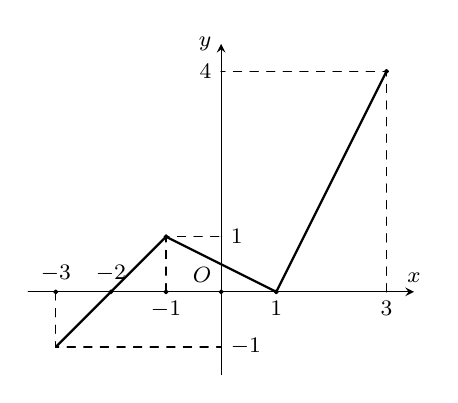
\begin{tikzpicture}[line cap=round, line join=round, font=\footnotesize, >=stealth, scale=0.7]
			\tikzset{label style/.style={font=\footnotesize}}
			\draw[->] (-3.5,0)--(3.5,0) node[above]{$x$};
			\draw[->] (0,-1.5)--(0,4.5) node[left]{$y$};
			\draw [thick] (-3,-1)--(-1,1)--(1,0)--(3,4);
			\draw[dashed] (-3,0)--(-3,-1)--(0,-1) (3,0)--(3,4)--(0,4) (-1,0)--(-1,1)--(0,1);
			\draw[fill=black] (0,0) circle (1pt) node[above left]{$O$}
			(1,0) circle (1pt) node[below]{$1$}
			(-1,0) circle (1pt) node[below]{$-1$}
			(-2,0) circle (1pt) node[above]{$-2$}
			(-3,0) circle (1pt) node[above]{$-3$}
			(0,1) circle (0pt) node[right]{$ 1 $} 
			(0,-1) circle (0pt) node[right]{$ -1 $} 
			(0,4) circle (0pt) node[left]{$ 4 $} 
			(3,0) circle (0pt) node[below]{$ 3 $} (3,4) circle (1pt) (-1,1) circle (1pt)
			;		
		\end{tikzpicture}
	\end{center}
	\choice
	{Đồ thị hàm số đi qua điểm $A(-3 ; 1)$}
	{Đồ thị cắt trục hoành tại 3 điểm phân biệt}
	{Hàm số nghịch biến trên $(-2 ; 1)$}
	{\True Hàm số đồng biến trên $(-3 ;-1)$ và $(1 ; 3)$}
	\loigiai{
		Theo hình vẽ ta thấy đồ thị hàm số đi lên từ trái sang phải (tăng) trên hai khoảng  $(-3 ;-1)$ và $(1 ; 3)$.	
	}
\end{ex}

\begin{ex}%Câu 19 %[0D1H1-5]%[Dự án đề kiểm tra Toán 10 GHKI NH23-24- Nguyễn Văn Sơn]%[THPT Tân Bình ]
	Cho mệnh đề $P(x):''\forall x \in \mathbb{R}, x^{2}+x+1>0 ''$. Mệnh đề phủ định của $P(x)$ là: 
	\choice
	{''$\forall x \in \mathbb{R}, x^{2}+x+1 \leq 0$''}
	{''$\forall x \in \mathbb{R}, x^{2}+x+1<0$''}
	{\True ''$\exists x \in \mathbb{R}, x^{2}+x+1 \leq 0^{\prime \prime}$''}
	{''$x \in \mathbb{R}, x^{2}+x+1>0$''}
	\loigiai{
		Mệnh đề $P(x):''\forall x \in \mathbb{R}, x^{2}+x+1>0 ''$ có mệnh đề phủ định là ''$\exists x \in \mathbb{R}, x^{2}+x+1 \leq 0^{\prime \prime}$''.
	}
\end{ex}

\begin{ex}%Câu 20 %[0D1N3-4]%[Dự án đề kiểm tra Toán 10 GHKI NH23-24- Nguyễn Văn Sơn]%[THPT Tân Bình ]
	Phần bù của tập $[-2 ; 1)$ trong $\mathbb{R}$ là
	\choice
	{$(2 ;+\infty)$}
	{$(-\infty ; 1]$}
	{$(-\infty ;-2)$}
	{\True $(-\infty ;-2) \cup[1 ;+\infty)$.}
	\loigiai{	
	}
\end{ex}


\begin{ex}%Câu 21 %[0H4V3-2]%[Dự án đề kiểm tra Toán 10 GHKI NH23-24- Nguyễn Văn Sơn]%[THPT Tân Bình ]
	Từ vị trí $A$ người ta quan sát một cây cao. Biết $A H=4 \mathrm{~m}, H B=20 \mathrm{~m}, \widehat{B A C}=45^{\circ}$. Khi đó chiều cao của cây là (tính chính xác đến hàng phần chục).
	\begin{center}
		\definecolor{lightcornflowerblue}{rgb}{0.6, 0.81, 0.93}
		\definecolor{cadmiumgreen}{rgb}{0.0, 0.42, 0.24}
		\definecolor{trueblue}{rgb}{0.0, 0.45, 0.81}
		\definecolor{tumbleweed}{rgb}{0.87, 0.67, 0.53}%màu cát
		
		\definecolor{forestgreen(web)}{rgb}{0.13, 0.55, 0.13}
		\definecolor{darkpastelgreen}{rgb}{0.01, 0.75, 0.24}
		\definecolor{bronze}{rgb}{0.8, 0.5, 0.2}
		\begin{tikzpicture}[line join=round, line cap=round,scale=1.5,transform shape]
			\clip (-4,-2.5) rectangle (4,2.5);
			\tikzset{cay/.pic={
					\def\T{ %Thân
						(-.33,0)%trái
						..controls +(-50:.25) and +(40:.45) ..  (-.57,-1.45)
						..controls +(20:.1) and +(-160:.15) ..  (-.1,-1.3)
						..controls +(-120:.1) and +(60:.15) ..  (-.2,-1.6)
						..controls +(-30:.1) and +(-140:.15) ..  (.15,-1.3)
						..controls +(-20:.1) and +(-160:.15) ..  (.57,-1.4)
						..controls +(170:.4) and +(-160:.1) ..  (.35,0)
						..controls +(110:.5) and +(80:.5) ..  (-.33,0)
						;}
					%\draw \T;
					\fill[bronze] \T;
					\def\C{ 
						(0,.3)
						..controls +(-100:.25) and +(-60:.2) ..  (-.3,.1)
						..controls +(-100:.25) and +(-60:.2) ..  (-.6,0)
						..controls +(-120:.45) and +(-110:.35) ..  (-1,.2)
						..controls +(-150:.5) and +(-140:.35) ..  (-1.15,.7)%nút giao
						..controls +(-170:.4) and +(-170:.35) ..  (-1,1.15)
						..controls +(140:.35) and +(110:.4) ..  (-.37,1.35)
						..controls +(110:.25) and +(80:.3) ..  (-.15,1.35)
						..controls +(80:.3) and +(95:.8) ..  (.55,1.1)
						..controls +(80:.2) and +(95:.2) ..  (.8,1.1)
						..controls +(20:.1) and +(95:.1) ..  (.95,1)
						..controls +(-20:.4) and +(35:.25) ..  (1,.47)
						..controls +(-30:.3) and +(-20:.3) ..  (.75,0.05)%nút giao
						..controls +(-120:.3) and +(-60:.2) ..  (.35,0)
						..controls +(175:.2) and +(-160:.1) ..  (.2,0.2)
						..controls +(-160:.1) and +(-70:.1) ..  (0,.3)
						;}
					\draw \C;
					\fill[forestgreen(web)] \C;
					\def\C1{ 
						(-1.15,.7)%nút giao
						..controls +(-170:.4) and +(-170:.35) ..  (-1,1.15)
						..controls +(140:.35) and +(110:.4) ..  (-.37,1.35)
						..controls +(110:.25) and +(80:.3) ..  (-.15,1.35)
						..controls +(80:.3) and +(95:.8) ..  (.55,1.1)
						..controls +(80:.2) and +(95:.2) ..  (.8,1.1)
						..controls +(20:.1) and +(95:.1) ..  (.95,1)
						..controls +(-20:.4) and +(35:.25) ..  (1,.47)
						..controls +(-50:.5) and +(-85:.6) ..  (.65,.55)% gần nút giao
						..controls +(-160:.4) and +(-120:.4) ..  (0,.7)
						..controls +(-150:.2) and +(-80:.4) ..  (-.63,.6)
						..controls +(-140:.5) and +(-130:.4) ..  (-1.15,.7)
						;}
					%\draw \C1;
					\fill[darkpastelgreen] \C1;
					\def\G{ %Gân
						(-.8,.2)
						..controls +(-35:.1) and +(130:.35) ..  
						(-.32,0)%nút giao
						..controls +(-40:.1) and +(45:.35) ..  (-.42,-1.25)
						(-.32,0)%nút giao
						..controls +(120:.1) and +(-45:.35) ..  (-.58,.45)
						(-.32,0)%nút giao
						..controls +(80:.1) and +(-170:.35) ..  (-.05,.45)
						(-.28,.3)
						..controls +(80:.1) and +(-60:.05) ..  (-.35,.55)
						%Gân phải
						(.45,-1.3)
						..controls +(130:.6) and +(-160:.3) ..  (.6,0.35)
						(.37,0)
						..controls +(35:.2) and +(-150:.1) ..  (.66,0.15)
						(.37,0)
						..controls +(80:.2) and +(-40:.1) ..  (.18,0.4)
						(.31,0.25)
						..controls +(80:.1) and +(-150:.1) ..  (.38,0.5)
						(.25,-0.15)
						..controls +(-110:.05) and +(110:.05) ..  (.2,-0.5)%gân dọc
						(.2,-0.25)
						..controls +(-110:.05) and +(110:.05) ..  (.17,-0.45)
						(-.2,-0.15)
						..controls +(-70:.1) and +(110:.05) ..  (-.18,-0.5)
						(-.15,-0.15)
						..controls +(-70:.1) and +(110:.05) ..  (-.15,-0.7)
						(-.05,-0.8)
						..controls +(-80:.15) and +(-10:.15) ..  (-.3,-1.28)
						(-.1,-0.9)
						..controls +(-110:.1) and +(20:.05) ..  (-.2,-1.1)
						(.1,-1)
						..controls +(-50:.05) and +(120:.05) ..  (.15,-1.2)
						(.1,-1.15)
						..controls +(-50:.05) and +(120:.05) ..  (.12,-1.2)
						(.15,-.75)
						..controls +(-120:.1) and +(-140:.1) ..  (.22,-.9)
						..controls +(70:.12) and +(120:.05) ..  (.18,-.9)
						;}
					
					\draw \G;
					
			}}
			
			\path
			(2,0)pic[scale=.8]{cay}	;
			\path 	(2,-1.1) coordinate (B)
			(-2,-1.1) coordinate (H)
			(-2,-.5) coordinate (A)
			(2,1.25) coordinate (C)	;
			\node at (B) [below]{\tiny $B$};
			\node at (H) [below]{\tiny $H$};
			\node at (A) [left]{\tiny $A$};
			\node at (C) [above]{\tiny $C$};
			\node at (-2,-.8) [left]{\tiny $4$};
			\node at (0,-1.1) [below]{\tiny $20$};
			\draw (B)--(H)--(A)--(C) (A)--(B);
			\draw    pic["\tiny $45^\circ$", draw=black, angle eccentricity=1.8, mark=1,angle radius=.4cm, color=blue]
			{angle=B--A--C};
			\draw    pic[draw=black, angle radius=.1cm]
			{right angle=A--H--B}; 
		\end{tikzpicture}
	\end{center}
	\choice
	{\True $ 17,3 \mathrm{~m} $}
	{$ 17,6 \mathrm{~m} $}
	{$ 17,9 \mathrm{~m} $}
	{$ 17 \mathrm{~m} $}
	\loigiai{
		Tam giác $ AHB $ vuông tại $ H $ nên ta có $ AB=\sqrt{AH^2+HB^2}=\sqrt{4^2+20^2}=4\sqrt{26} \mathrm{~m}. $\\
		Ta có $ \tan \widehat{HAB}=\dfrac{BH}{AH}=5\Rightarrow \widehat{HAB}\approx 78{,}7^\circ$.\\
		Ta lại có $ AH \parallel BC \Rightarrow \widehat{ABC}=\widehat{HAB}\approx 78{,}7^\circ\Rightarrow \widehat{ACB}=180^\circ-\widehat{CAB}-\widehat{ABC}\approx 56{,}3^\circ $.\\
		Áp dụng định lý sin trong tam giác $ ABC $ ta có \\
		$\dfrac{BC}{\sin\widehat{BAC}}=\dfrac{AB}{\sin\widehat{ACB}}\Rightarrow BC = \dfrac{AB}{\sin\widehat{ACB}}\cdot \sin\widehat{BAC}\approx 17{,}3 \mathrm{~m}$.
		
	}
\end{ex}

\begin{ex}%Câu 22[0D1H2-2]% %[Dự án đề kiểm tra Toán 10 GHKI NH23-24- Nguyễn Văn Sơn]%[THPT Tân Bình ]
	Cho hai tập hợp $A=\{1 ; 2 ; 5 ; 7\}, B=\{1 ; 2 ; 3\}$. Có bao nhiêu tập hợp $X$ thỏa mãn $X \subset A$ và $X \subset B$.
	\choice
	{$ 3 $ }
	{$ 1 $}
	{$ 4 $ }
	{$ 2 $}
	\loigiai{
		Các tập $ X $ thỏa là: $ \varnothing, \{1\}, \{2\}, \{1; 2\} $. Do đó có $ 4 $ tập $ X $ thỏa đề bài.
	}
\end{ex}

\begin{ex}%Câu 23 %0D1V3-5%[Dự án đề kiểm tra Toán 10 GHKI NH23-24- Nguyễn Văn Sơn]%[THPT Tân Bình ]
	Trong số $ 35 $ học sinh của lớp $ 10A $, có $ 20 $ học sinh thich môn Toán, $ 16 $ học sinh thích môn Tiếng Anh và $ 12 $ học sinh thích cả hai môn này. Hỏi lớp $10 A$ có bao nhiêu học sinh không thích cả hai môn này?
	\choice
	{$ 36 $}
	{$ 12 $}
	{$ 24 $}
	{\True $ 11 $}
	\loigiai{
		Đặt $ A $ là tập các học sinh thích Toán. Suy ra $ n(A)=20. $\\
		$ B $ là tập các học sinh thích Tiếng Anh. Suy ra $ n(B)=16 $.\\
		Khi đó $ A\cap B $ là số học sinh thích cả hai môn và $ n(A\cap B)=12 $.\\
		Tập học sinh có thích Toán hoặc Tiếng Anh là $ A\cup B $.\\
		Ta có công thức $ n(A\cup B)=n(A)+n(B)+n(A\cap B)=20+16-12=24 $.\\
		Suy ra số học sinh không thích cả hai môn này là $ 35-24=11 $ học sinh.
	}
\end{ex}

\begin{ex}%Câu 24 %[0H4K2-2]%[Dự án đề kiểm tra Toán 10 GHKI NH23-24- Nguyễn Văn Sơn]%[THPT Tân Bình ]
	Cho hình bình hành $ABCD$ có $AB=a, BC=a \sqrt{2}$ và $\widehat{BAD}=135^{\circ}$. Diện tích của hình bình hành $ABCD$ bằng
	\choice
	{$2a^{2}$}
	{\True $a^{2}$}
	{$a^{2}\sqrt{2}$}
	{$a^{2}\sqrt{3}$}
	\loigiai{
		Ta có $ AD\parallel BC $ nên $ \widehat{ABC}+\widehat{BAD}=180^\circ $ (kề bù).\\
		Suy ra $ \widehat{ABC}=180^\circ - \widehat{BAD}=45^\circ $.\\
		Diện tích hình bình hành $ ABCD $ là $ S=AB.BC.\sin\widehat{ABC}=a.a\sqrt{2}.\sin 45^\circ = a^2$.
	}
\end{ex}

\Closesolutionfile{ans}

\begin{center}
	\textbf{PHẦN 2 - TỰ LUẬN}
\end{center}

%Câu 1...........................
\begin{bt}%ID%[Dự án đề kiểm tra Toán 10 GHKI NH23-24- Tacgia]%[THPT ]
Cho hai tập hợp $A=(-2;2]$ và $B=[1;5)$. Xác định các tập hợp $A\cup B,A\cap B, B\setminus A,C_{\mathbb{R}}B$.
\loigiai{
	\begin{center}
		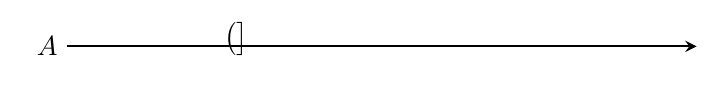
\begin{tikzpicture}[thick,>=stealth]
			\draw[->](-2,0)node[shift={(180:7pt)}]{$A$}->(6,0);
			\IntervalLR{-2}{-1}
			\def\skipInterval{0.5cm}
			\IntervalGRF{}{}{\big(}{-2}
			\IntervalLR{2}{6}
			\def\skipInterval{0.5cm}
			\IntervalGRF{\big]}{2}{}{}
		\end{tikzpicture}\\
		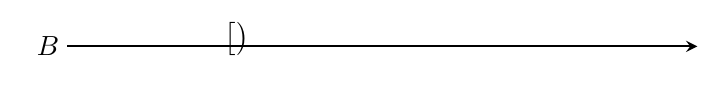
\begin{tikzpicture}[thick,>=stealth]
			\draw[->](-2,0)node[shift={(180:7pt)}]{$B$}->(6,0);
			\IntervalLR{-2}{.5}
			\def\skipInterval{0.5cm}
			\IntervalGRF{}{}{\big[}{1}
			\IntervalLR{5}{6}
			\def\skipInterval{0.5cm}
			\IntervalGRF{\big)}{5}{}{}
		\end{tikzpicture}
	\end{center}
	Dựa vào hình vẽ, ta có
	\begin{itemize}
		\item $A\cup B=(-2;5)$.
		\item $A\cap B=[1;2]$.
		\item $B\setminus A=(-2;1)$.
		\item $C_{\mathbb{R}}B=\mathbb{R}\setminus B=(-\infty;1)\cup [5;+\infty)$.
	\end{itemize}
}
\end{bt}
%Câu 2...........................
\begin{bt}%ID%[Dự án đề kiểm tra Toán 10 GHKI NH23-24- Tacgia]%[THPT ]
	Xét tính đồng biến và nghịch biến của hàm số $f(x)=2x^2-7$ trên khoảng $(2;5)$.
	\loigiai{
		Hàm với xác định định với mọi $x\in\mathbb{R}$. Suy ra nó xác định trên khoảng $(2;5)$.\\
		Lấy $x_1,x_2$ là hai số túy ý thuộc khoảng $(2;5)$ sao cho $2<x_1<x_2<5$, ta có \[f(x_1)-f(x_2)=(2x_1^2-7)-(2x_2^2-7)=2(x_1-x_2)(x_1+x_2).\]
		Do $2<x_1<x_2<5$ nên $x_1-x_2<0$. Suy ra $f(x_1)-f(x_2)<0$ hay $f(x_1)<f(x_2)$.\\
		Vậy hàm số đã cho đồng biến trên khoảng $(2;5)$.
	}
\end{bt}
%Câu 3...........................
\begin{bt}%ID%[Dự án đề kiểm tra Toán 10 GHKI NH23-24- Tacgia]%[THPT ]
	\immini{Từ vị trí $A$ cách mặt đất $1$ mét, một bạn nhỏ quan sát một cây đèn đường theo hình vẽ sau.
		Biết $HB$ bằng $6$ mét, góc $\widehat{BAC}=44^\circ$. Khoảng cách từ mắt của bạn đến mặt đất là $1$ mét. Hãy tính chiều cao của cây đèn đường (kết quả làm tròn đến $1$ chữ số thập phân).}
	{\begin{tikzpicture}[scale=1, font=\footnotesize, line join=round, line cap=round, >=stealth]
			\path
			(0,0) coordinate (H)
			(5,0) coordinate (B)
			(0,1) coordinate (A)
			(5,3.8) coordinate (C);
			\path ($(B)!.48!(C)$) node	{\begin{tikzpicture}
					\draw plot coordinates{(0,0)(-.5,0) (-0.31,0.39) (-0.2,0.39) (-0.2,2.52)(-0.31,2.52) (-0.31,2.76) (-0.22,2.76)(-0.11,3.12)(0,3.8)};
					\fill[violet] plot coordinates{(0,0)(.5,0) (0.31,0.39) (0.2,0.39) (0.2,2.52)(0.31,2.52) (0.31,2.76) (0.22,2.76)(0.11,3.12)(0,3.8)};
				\end{tikzpicture}
			};
			\draw (B)--(H)--(A) (C)--(A)--(B);
			\draw
			pic[draw,angle eccentricity=1.1,"$44^\circ$",right,angle radius=.6cm] {angle=B--A--C};
			\foreach \x/\g in{A/180,B/-90,C/90,H/-90} \draw[fill=black] (\x) circle (.05)+(\g:.4) node {$\x$};
			\path 
			($(H)!.5!(A)$) node[left]{$1 \text{\,m}$}
			($(H)!.5!(B)$) node[below] {$6 \text{\,m}$};
	\end{tikzpicture}}
	\loigiai{		
	\immini{Tam giác $ABD$ vuông tại $D$ có $\tan \widehat{BAD}=\dfrac{BD}{AD}=\dfrac{1}{6}\\
		\Rightarrow \widehat{BAD}\approx 9^\circ 28'\Rightarrow \widehat{DAC}=34^\circ 32'$.\\
		Tam giác $ADC$ vuông tại $D$ có \[CD=AD\cdot \tan 34^\circ32'\approx 4{,}1\,\mathrm{m}.\]
		Vậy chiều cao của cây đèn đường là $4{,}1+1=5{,}1\,\mathrm{m}$.
	}
	{\begin{tikzpicture}[scale=1, font=\footnotesize, line join=round, line cap=round, >=stealth]
			\path
			(0,0) coordinate (H)
			(5,0) coordinate (B)
			(5,1) coordinate (D)
			(0,1) coordinate (A)
			(5,3.8) coordinate (C)
			;
			\path ($(B)!.48!(C)$) node	{\begin{tikzpicture}
					\draw plot coordinates{(0,0)(-.5,0) (-0.31,0.39) (-0.2,0.39) (-0.2,2.52)(-0.31,2.52) (-0.31,2.76) (-0.22,2.76)(-0.11,3.12)(0,3.8)};
					\fill[violet] plot coordinates{(0,0)(.5,0) (0.31,0.39) (0.2,0.39) (0.2,2.52)(0.31,2.52) (0.31,2.76) (0.22,2.76)(0.11,3.12)(0,3.8)};
				\end{tikzpicture}
			};
			\draw (B)--(H)--(A)--(D)--(B)--(A) (C)--(A)--(D);
			\draw
			pic[draw,angle eccentricity=1.1,angle radius=.2cm] {right angle=A--D--C}
			pic[draw,angle eccentricity=1.1,"$44^\circ$",right,angle radius=.6cm] {angle=B--A--C};
			\foreach \x/\g in{A/180,B/-90,C/90,D/0,H/-90} \draw[fill=black] (\x) circle (.05)+(\g:.4) node {$\x$};
			\path 
			($(H)!.5!(A)$) node[left]{$1 \text{\,m}$}
			($(H)!.5!(B)$) node[below] {$6 \text{\,m}$};
	\end{tikzpicture}}
	}
\end{bt}
%Câu 4...........................
\begin{bt}%ID%[Dự án đề kiểm tra Toán 10 GHKI NH23-24- Tacgia]%[THPT ]
	Một nhân viên bán hàng sẽ nhận được mức lương cơ bản  là $5$ triệu đồng mỗi tháng và khoản hoa hồng là $5\%$ nếu tổng doanh thu trên $10$ triệu đồng trong tháng. Ngoài ra nếu nếu doanh thu bán hàng hàng tháng là $20$ triệu đồng hoặc nhiều hơn thì nhân viên bán hàng nhận được thêm tiền thưởng là $500.000$ đồng.
	\begin{enumerate}
		\item Hãy biểu diễn thu nhập hàng tháng của nhân viên bằng một hàm số theo doanh thu bán hàng.
		\item Nếu doanh thu trong một tháng của nhân viên đó là $30$ triệu đồng thì nhân viên sẽ nhận được ba nhiêu tiền lương?
	\end{enumerate}
	\loigiai{
		\begin{enumerate}
			\item $f(x)=\heva{&5&\text{ khi }&0\le x\le 10\\&5+5\%x&\text{ khi }&10\le x< 20\\&5{,}5+5\%x&\text{ khi }&x\ge 20}.$
			\item Khi $x=30$ triệu đồng thì nhân viên sẽ nhận được ba nhiêu tiền lương là \[f(30)=5{,}5+5\%\cdot 30=7\text{ (triệu đồng).}\]
		\end{enumerate}
	}
\end{bt}
\begin{center}
	\textbf{ĐÁP ÁN}
	\inputansbox{10}{ans/ans}	
\end{center}